% Section 5: Analysis
% Note: \section{} header is in main.tex

\subsection{Metric-Dependent Collapse: Format vs.\ Semantic}
\label{sec:format_vs_semantic}

\begin{figure}[t]
\centering
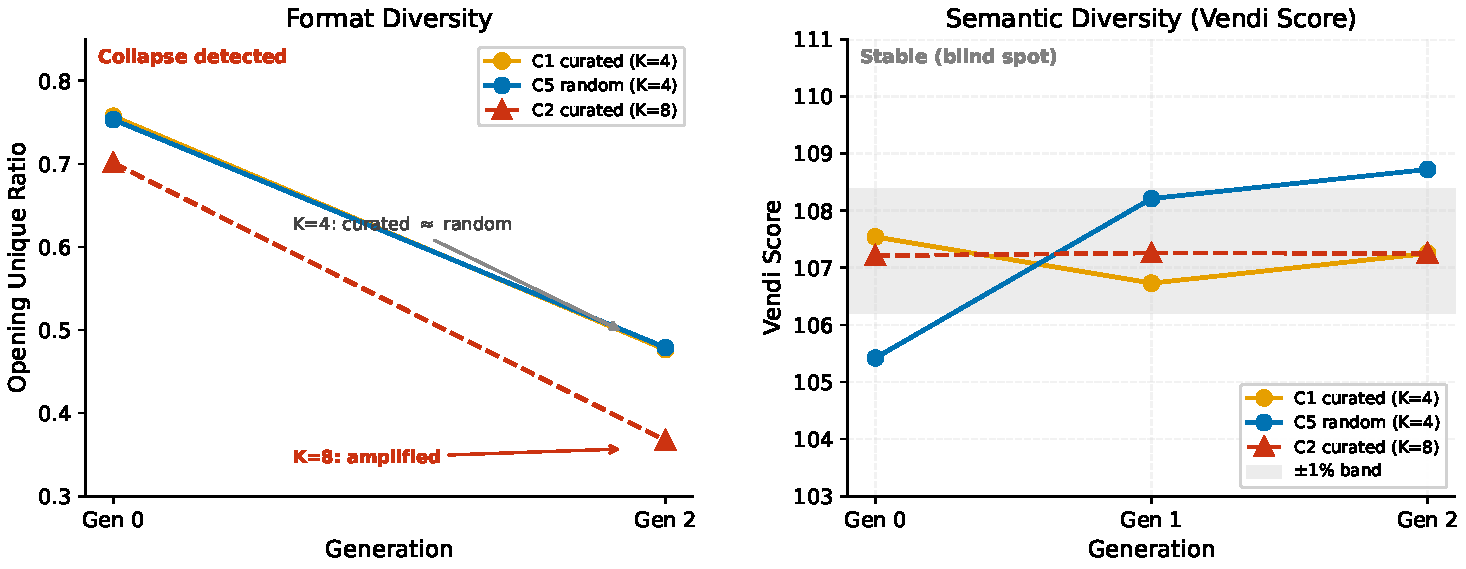
\includegraphics[width=\columnwidth]{figures/fig4_format_collapse.pdf}
\caption{Format diversity metrics across generations for LoRA $K{=}4$ curated (C1) and random baseline (C5). Both conditions show nearly identical format degradation, confirming that format collapse is driven by iterative self-training rather than reward curation.}
\label{fig:format_collapse}
\end{figure}

Diversity collapse under iterative self-training is real but mischaracterized by standard embedding-based metrics. Semantic diversity as measured by Vendi Score remains stable across generations (Section~\ref{sec:no_collapse}), yet surface-level formatting undergoes substantial homogenization. Table~\ref{tab:format_collapse} presents format diversity metrics for the LoRA $K{=}4$ curated condition (C1) and the LoRA $K{=}4$ random baseline (C5) across Gen~0 and Gen~2. Opening unique ratio, defined as the fraction of responses with a unique first 50 characters, drops from 0.757 to 0.477 under curation and from 0.753 to 0.479 under the random baseline. Opening entropy (Shannon entropy over first-10-token sequences, in bits) declines by 0.75 bits under both conditions. The near-duplicate start rate (fraction of responses sharing a 50-character prefix with at least one other response) rises from 37.9\% to 75.6\% under curation and from 38.3\% to 74.9\% under the baseline. Both conditions exhibit nearly identical degradation trajectories (Figure~\ref{fig:format_collapse}), which indicates that format collapse is an intrinsic property of iterative self-training rather than a consequence of reward curation. The C2 condition ($K{=}8$) provides further evidence: its opening entropy drops by 1.13 bits, compared to 0.75 bits for both $K{=}4$ conditions. Doubling $K$ amplifies homogenization, which suggests that candidate pool size acts as a scaling factor for format collapse. More candidates per prompt increase the probability of selecting responses that share common structural patterns and thereby reinforce template convergence across generations.

\begin{table}[t]
\centering
\small
\caption{Format diversity metrics for LoRA $K{=}4$ curated (C1) and LoRA $K{=}4$ random baseline (C5). Both conditions show nearly identical degradation across all metrics, which confirms that format collapse is driven by iterative self-training rather than reward curation.}
\label{tab:format_collapse}
\resizebox{\columnwidth}{!}{%
\begin{tabular}{@{}lcccc@{}}
\toprule
Metric & C1 Gen~0 & C1 Gen~2 & C5 Gen~0 & C5 Gen~2 \\
\midrule
Opening unique ratio & 0.757 & 0.477 & 0.753 & 0.479 \\
Opening entropy (bits) & 12.43 & 11.68 & 12.43 & 11.68 \\
Near-dup start rate (\%) & 37.9 & 75.6 & 38.3 & 74.9 \\
Per-response TTR & 0.682 & 0.670 & 0.683 & 0.660 \\
Trigram repetition rate & 0.174 & 0.256 & 0.174 & 0.258 \\
\bottomrule
\end{tabular}}
\end{table}

The mechanism is self-reinforcing: when a model trains on its own outputs, frequent structural patterns are overrepresented in the training data, the fine-tuned model generates these patterns more often, and the cycle repeats. This loop operates on surface formatting while leaving semantic content untouched, regardless of whether training data is reward-curated or random. Per-response type-token ratio (TTR) drops by only 0.012 under curation compared to 0.023 under random, confirming that the effect is confined to structural formatting rather than vocabulary.

The Vendi Score's insensitivity has a technical explanation: the sentence embeddings (all-MiniLM-L6-v2) encode semantic content and are largely invariant to surface formatting. Two responses with identical openings but different topics receive distant embeddings. This disconnect means Vendi Score alone provides an incomplete picture of how iterative training reshapes the output distribution.

\subsection{Why Semantic Collapse Does Not Occur}
\label{sec:why_no_collapse}

We hypothesize three contributing factors that together account for the observed semantic stability. First, \textbf{prompt diversity} acts as an external anchor: 2{,}200 diverse prompts force broad semantic coverage at every generation regardless of per-prompt selection. Second, \textbf{reward model saturation} limits selection pressure. The ArmoRM score gap between top-1 and pool average is approximately 0.04, so the curated candidate differs only marginally from a random alternative. Third, \textbf{generation stochasticity} ($T{=}0.7$) injects fresh variation at each iteration, counteracting convergence to fixed outputs.

These factors connect to the sufficient conditions for model collapse identified by \citet{placeholder_shumailov}: progressive distribution narrowing requires that synthetic data fully replaces external data and that sampling does not introduce compensating variance. In our setup, prompt diversity violates the first condition (an external scaffold persists across generations), and stochastic decoding violates the second. Reward saturation further weakens the selection channel through which curation could compound. C8 ($K{=}16$, 6.25\% retention) provides the strongest test: under four times the selection pressure of $K{=}4$ configurations, Vendi Score changes by only $-$0.19\% while training loss falls to 0.097. Even when curation retains fewer than 1 in 15 candidates, the semantic distribution remains stable. Isolating the individual contribution of each factor (e.g., through controlled ablation of prompt diversity or decoding temperature) remains an important direction for future work.

\subsection{LoRA as Capacity Bottleneck}
\label{sec:lora_bottleneck}

The similarity of diversity outcomes between $K{=}4$ and $K{=}8$ LoRA conditions despite doubled selection pressure suggests that parameter capacity, not curation intensity, is the binding constraint under LoRA. The rank-16 adapter modifies only 1.67\% of parameters, limiting how far any training signal can reshape the output distribution (see Appendix~\ref{app:lora_bottleneck} for detailed analysis).

\subsection{Implications for Diversity Measurement}
\label{sec:measurement_implications}

Standard diversity evaluation relies on embedding-based metrics that are insensitive to format-level homogenization. Our results show this workflow misses an entire dimension of collapse visible to human readers.

We propose two complementary metrics: \emph{opening entropy} (Shannon entropy over first-10-token sequences) and \emph{near-duplicate start rate} (fraction sharing a 50-character prefix). Both require only string operations, need no GPU, and capture a failure mode orthogonal to semantic metrics. In our experiments, opening entropy drops 0.75 bits at $K{=}4$ (1.13 bits at $K{=}8$) while Vendi Score changes by only $-$0.27\%, and near-duplicate start rate rises 38 pp while Self-BLEU remains below 0.007.

The broader lesson is that ``diversity'' in iterative self-training is not a single quantity. Format, semantic, and lexical diversity can evolve independently under the same procedure. A complete diversity audit should include at least one metric from each dimension.